% 
%            ,,                                        
%          `7MM            _.o9                                
%            MM                                             
%  ,6"Yb.    MM  ,p6"bo   ,6"Yb.  M"""MMV  ,6"Yb.  `7Mb,od8 
% 8)   MM    MM 6M'  OO  8)   MM  '  AMV  8)   MM    MM' "' 
%  ,pm9MM    MM 8M        ,pm9MM    AMV    ,pm9MM    MM     
% 8M   MM    MM YM.    , 8M   MM   AMV  , 8M   MM    MM     
% `Moo9^Yo..JMML.YMbmd'  `Moo9^Yo.AMMmmmM `Moo9^Yo..JMML.   
% 
% 
% Free and Open-Source template for academic works
% https://github.com/dpmj/alcazar

\newpage


\clearpage
\cleardoublepage
\phantomsection

\pagestyle{empty}

\phantomsection
\addcontentsline{toc}{chapter}{About this work}


%%%%%%%%%%%%%%%%%%%%%%%%%%%%%%%%%%%%%%%%%%%%%%%%%%%%%%%%%%%%%%%%%%%%%%%%%%%%%%%%%%%%%%%%%%%%
% ABOUT THE AUTHORS

\begingroup

    \small
    \setlength\tabcolsep{0pt}
    \renewcommand*{\arraystretch}{1}
    
    \noindent
    \begin{tabular}{p{3.5cm} p{11.5cm}}
        \vspace{0mm} 
\includegraphics[width=3cm]{opening/resources/about/kleiner.png} & \vspace{-0.5mm} {\large \thesisAuthor} 
        \newline A short paragraph about you and how handsome and hard-working you are. Brag about your work, awards, publications and merits. The glory is yours! Congratulations. The Lorem ipsum dolor sit amet, consectetur adipiscing elit. Integer tempus quis elit id sagittis. Cras tincidunt nisi at tellus luctus, et congue dolor posuere. Aliquam suscipit felis sit amet lacus ultrices aliquet. Sed sagittis ultrices nisi, vel elementum elit dignissim non. 
        \vspace{2mm} 
        \newline
        \href{https://orcid.org/}{  % Link to your orcid
            \icon{\faOrcid}{10}{orcid-green}
        }
        \href{https://www.linkedin.com/}{  % Link to your linkedin
            \icon{\faLinkedinIn}{10}{linkedin-blue}
        }
        \href{https://github.com/}{  % Link to your github
            \icon{\faGithub}{10}{github-black}
        }
        \href{https://twitter.com/}{  % Link to your twitter
            \icon{\faTwitter}{10}{twitter-blue}
        }
        \href{mailto:example@domain.org}{  % Your E-mail
            \icon{\faEnvelope}{10}{email-red}
        }
        \href{https://t.me/}{  % Link to your telegram
            \icon{\faTelegramPlane}{10}{telegram-blue}
        }
    \end{tabular}
    
    \vspace{10mm}
    
    \noindent
    \begin{tabular}{p{3.5cm} p{11.5cm}}
        \vspace{0mm} 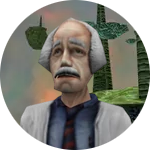
\includegraphics[width=3cm]{opening/resources/about/coomer.png} & \vspace{-0.5mm} {\large \thesisTutor} 
        \newline What a big fish you've got yourself. Show off your tutor. Now that's a job well done. Lorem ipsum dolor sit amet, consectetur adipiscing elit. Integer tempus quis elit id sagittis. Cras tincidunt nisi at tellus luctus, et congue dolor posuere. Aliquam suscipit felis sit amet lacus ultrices aliquet. Sed sagittis ultrices nisi, vel elementum elit dignissim non. Fusce faucibus ex at massa ultrices elementum.
        \vspace{2mm} 
        \newline
        \href{https://orcid.org/}{  % Link to your orcid
            \icon{\faOrcid}{10}{orcid-green}
        }
        \href{https://www.linkedin.com/}{  % Link to your linkedin
            \icon{\faLinkedinIn}{10}{linkedin-blue}
        }
        \href{https://github.com/}{  % Link to your github
            \icon{\faGithub}{10}{github-black}
        }
        \href{https://twitter.com/}{  % Link to your twitter
            \icon{\faTwitter}{10}{twitter-blue}
        }
        \href{mailto:example@domain.org}{  % Your E-mail
            \icon{\faEnvelope}{10}{email-red}
        }
        \href{https://t.me/}{  % Link to your telegram
            \icon{\faTelegramPlane}{10}{telegram-blue}
        }
    \end{tabular}
    
\endgroup





%%%%%%%%%%%%%%%%%%%%%%%%%%%%%%%%%%%%%%%%%%%%%%%%%%%%%%%%%%%%%%%%%%%%%%%%%%%%%%%%%%%%%%%%%%%%
% how to cite this work

% Listings workaround to include the background in broken lines

% \begin{verbatimwrite}{cite.txt}
% @mastersthesis{citeKey,
%     author  = "(*@{\thesisAuthor}@*) and (*@{\thesisTutor}@*)",
%     title   = "(*@{\thesisTitle}@*)",
%     school  = "(*@{\thesisSchool}@*)",
%     year    = "(*@{\thesisYear}@*)",
%     month   = "(*@{\thesisMonth}@*)",
%     address = "(*@{\thesisAddress}@*)"
% }
% \end{verbatimwrite}


\begingroup

\vspace*{\fill}

\small
\setlength\tabcolsep{0pt}
\renewcommand*{\arraystretch}{1.2}
{\noindent\large  Cite this work:}

% \begin{mdframed}[backgroundcolor=listing-background,hidealllines=true]
\vspace*{2mm}
% \lstinputlisting[style=cite, nolol]{./cite.txt}

\newwrite\tempfile
\immediate\openout\tempfile=cite.txt
\immediate\write\tempfile{%
@mastersthesis{citeKey,^^J
author  = "\thesisAuthor \space and \thesisTutor",^^J
title   = "\thesisTitle",^^J
school  = "\thesisSchool",^^J
year    = "\thesisYear",^^J
month   = "\thesisMonth",^^J
address = "\thesisAddress",^^J
type = "\thesisType"^^J
}
}
\immediate\closeout\tempfile

% Does not work because escapes are inside strings
% \begin{minted}{bibtex}
% @mastersthesis{citeKey,
%     author  = "¢{\thesisAuthor}¢ and ¢{\thesisTutor}¢",
%     title   = "¢{\thesisTitle}¢",
%     school  = "¢{\thesisSchool}¢",
%     year    = "¢{\thesisYear}¢",
%     month   = "¢{\thesisMonth}¢",
%     address = "¢{\thesisAddress}¢"
% }
% \end{minted}

\inputminted[style=algol_nu]{bibtex}{./cite.txt}
% \end{mdframed}


\endgroup
